\begin{figure}
	{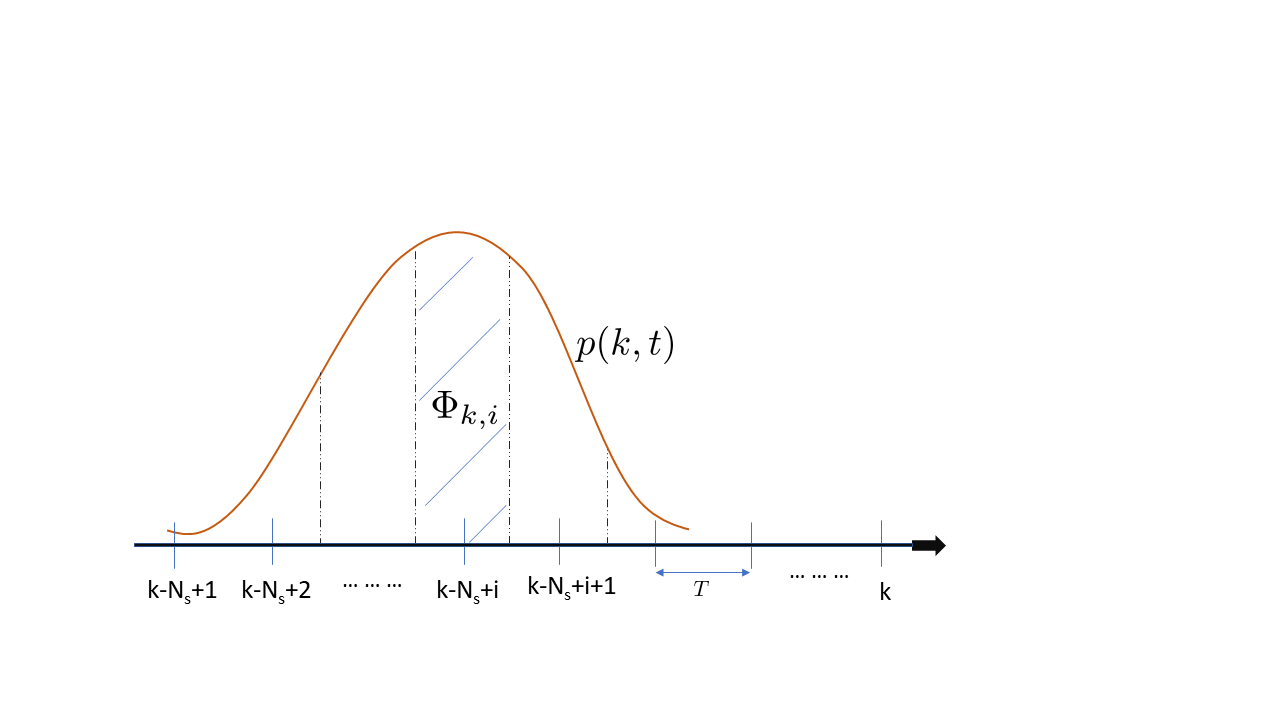
\includegraphics[width=1.0\columnwidth]{./img/delay_uncertainty.png}}
	\caption{Uncertianty of delay}
	\label{fig:delay_uncertainty}
\end{figure}

This section will describe the state estimation approach for the linear system in eqns. (\ref{eqn:LinearStatePropModel}) and (\ref{eqn:LinearUndelayedMeasurementModel}), along with time delayed measurements modelled in eqn. (\ref{eqn:LinearDelayedMeasurementModel}), which are corrupted by unknown bias $\Boldb_k$. 
For the derivation of the approach described in this section the reader is advised to refer to the Section IV in \cite{choi2012state}.

It is essential to known the value of bias to migitate its effect on the posterior estimate of the state. Since it's not known prior to the estmiation, $\Boldb_k$ is simultaneously estimated along with the state. 
Assume that state vector at time $k$ is denoted by $\Boldtheta_k$.
The simultaneous estimation of the state \& the bias is achieved by performaning estimation over an updated state vector 
\begin{equation}
	\Boldx_k =
	\begin{bmatrix}
		\Boldtheta_k \\ \Boldb_k
	\end{bmatrix}. 
\end{equation}

The probability density function (PDF) $p(t)$ of the delay is assumed to be a known. As shown in figure (\ref{fig:delay_uncertainty}) the pdf is assumed to span over $N_{max}$ time steps. This assumption assigns a probability for correspondence of the delayed measurement $\Boldz_k$ with each of the time steps within time step $k$ and $k- N_{max}$.
Correspondence $\phi(k,i)$, $\forall i \in \{0, \dots, N_{max}\}$, signifies that measurement $\Boldz_k$ was induced by the state $\Boldx_{k-N_{max}+i}$.
The probability of correpondence $\phi_i$ is computed as
\begin{align}
	\Phi_{k,i} &= P(\phi(k,i)) \\
	&= P(t_l \le t \le t_u) \\
	&= \int_{t_l}^{ t_u} p(t) dt,
\end{align}
where $t_l = {j\tau - \frac{\tau}{2}}$, $t_u = {j \tau + \frac{\tau}{2}}$, $j = k - N_{max} + i $, $P(\cdot)$ denotes probability and $p(\cdot)$ denotes pdf of the time delay. When the PDF of the delay is specified, the maximum delay $N_{max}$ can be calculated using the cmulative distribution function (CDF) of the PDF. 
A value of $N_{max}$ should be chosen such that CDF of the time delay exceeds a given threshold. 
%A higher threshold value 99.6\% will ensure that the state $\Boldx_s$, where $k-N_{max} \le s \le k$, which induced the delayed measurement $\Boldz_k$ .
Choi et. al. have shown that probability of the correspondence $\phi_i$ for the given measurment $\Boldz_k$ is \cite{choi2012state}
\begin{align}
	P(\phi(k,i) | \Boldz_k ) = P(\phi(k,i)) = \Phi_{k,i}
\end{align}

Then, the optimal state estimator is
\begin{align}
	\hat{\Boldx}_k = \sum_{i=0}^{N_{max}} \Phi_{k,i} \hat{\Boldx}_{k,i},
\end{align}
where $\hat{\Boldx}_{k,i}$ denotes the state estimate $\hat{\Boldx}_j^+$ computed in eqn. (\ref{eqn:posterior_state_estimate}), where $j = k - N_{max} + i$.

The optimal covariance matrix of the estimate is
\begin{align}
	\BoldP_k = \sum_{i = 0}^{N_{max}} \Phi_{k,i} [\BoldP_{k,i} + \hat{\Boldx}_k \hat{\Boldx}_k^\top] - \hat{\Boldx}_k \hat{\Boldx}_k^\top	
\end{align}
where $\BoldP_{k,i}$ is $a~posteriori$ state covariance matrix $P_j^+$ computed in eqn. (\ref{eqn:posterior_state_covar}),  where $j = k - N_{max} + i$.



